\subsection{Why we use Flex and Bison tools for parsing?}

Flex and Bison are aging unix utilities that help you write very fast parsers for almost arbitrary file formats. Formally, they implement Look-Ahead-Left-Right (as opposed to "recursive descent") parsing of non-ambiguous context-free (as opposed to "natural language") grammars.\\
Why should you learn the Flex/Bison pattern syntax when you could just write your own parser? Well, several reasons. First, Flex and Bison will generate a parser that is virually guaranteed to be faster than anything you could write manually in a reasonable amount of time. Second, updating and fixing Flex and Bison source files is a lot easier than updating and fixing custom parser code. Third, Flex and Bison have mechanisms for error handling and recovery, which is something you definitely don't want to try to bolt onto a custom parser. Finally, Flex and Bison have been around for a long time, so they far freer from bugs than newer code.\\\\

\subsection{lex vs. flex, yacc vs. bison}
In addition to hearing about "flex and bison", you will also hear about "lex and yacc". "lex and yacc" are the original tools; "flex and bison" are their almost completely compatible newer versions. Only very old code uses lex and yacc; most of the world has moved on to Flex and Bison.\\
All four of the above are C-based tools; they're written in C, but more important their output is C code. However, my project was in C++ -- so this is also a tutorial on how to use C++ with Flex and Bison! \\\\

\subsection{flex: The Fast Lexical Analyzer}
Flex is a tool for generating scanners. A scanner, sometimes called a tokenizer, is a program which recognizes lexical patterns in text. The flex program reads user-specified input files, or its standard input if no file names are given, for a description of a scanner to generate. The description is in the form of pairs of regular expressions and C code, called rules. Flex generates a C source file named, "lex.yy.c", which defines the function yylex(). The file "lex.yy.c" can be compiled and linked to produce an executable. When the executable is run, it analyzes its input for occurrences of text matching the regular expressions for each rule. Whenever it finds a match, it executes the corresponding C code.
Flex and Bison files have three sections:\\\\
\begin{itemize}
\item The first is sort of "control" information
\item The second is the actual token/grammar definitions
\item The last is C/C++ code to be copied verbatim to the output
\end{itemize}

Flex file can be compiled by running this:\\\\
\begin{enumerate}
\item $ flex nameOfFlexFile $
\item $ g++ lex.yy.c -lfl -o outfilename $
\end{enumerate}



\begin{large}\subsection{Bison}\end{large}
Bison is a general-purpose parser generator that converts an annotated context-free gram-
mar into a deterministic LR or generalized LR (GLR) parser employing LALR(1) parser
tables. As an experimental feature, Bison can also generate IELR(1) or canonical LR(1)
parser tables. Once you are proficient with Bison, you can use it to develop a wide range
of language parsers, from those used in simple desk calculators to complex programming
languages.\\\\
Bison is upward compatible with Yacc: all properly-written Yacc grammars ought to
work with Bison with no change. Anyone familiar with Yacc should be able to use Bison
with little trouble. You need to be fluent in C or C++ programming in order to use Bison
or to understand this manual. Java is also supported as an experimental feature.\\\\
Bison was written originally by Robert Corbett. Richard Stallman made it Yacc-
compatible. Wilfred Hansen of Carnegie Mellon University added multi-character string
literals and other features.\\\\
\subsection{Main concepts of Bison}
\subsection{Languages and Context-Free Grammars}
In order for Bison to parse a language, it must be described by a context-free grammar.
This means that you specify one or more syntactic groupings and give rules for constructing
them from their parts. For example, in the C language, one kind of grouping is called an
‘expression’. One rule for making an expression might be, “An expression can be made of a
minus sign and another expression”. Another would be, “An expression can be an integer”.
As you can see, rules are often recursive, but there must be at least one rule which leads
out of the recursion.\\\\
\begin{figure} [h]
\centering

\includegraphics[scale=1.5]{images/bisondev.jpg}
\caption{Richard Stallman}
\end{figure}
The most common formal system for presenting such rules for humans to read is Backus-
Naur Form or “BNF”, which was developed in order to specify the language Algol 60. Any
grammar expressed in BNF is a context-free grammar. The input to Bison is essentially
machine-readable BNF.\\\\
In the formal grammatical rules for a language, each kind of syntactic unit or grouping
is named by a symbol. Those which are built by grouping smaller constructs according
to grammatical rules are called nonterminal symbols; those which can’t be subdivided
are called terminal symbols or token types. We call a piece of input corresponding to a
single terminal symbol a token, and a piece corresponding to a single nonterminal symbol
a grouping.\\\\


\subsection{DXF File Format}
The task of reading through the DXF library and rebuilding it, requires a great effort. At this stage I can’t think of re-writing the library as I new to it. Today, I have gone through the basics of DXF library. DXF is a file format used for importing and exporting 2-d drawings.\\
DXF stands for Drawing Exchange Format. Files that contain the .dxf file extension contain CAD vector image files. The DXF file format is similar to the DWG file format, but DXF files are ASCII based and are therefore more compatible with other computer applications.\\\\
The DXF file format was developed as an exchange format for the CAD files that are created by computer aided drafting software applications. The file format was initially introduced in December of 1982 as a part of AutoCAD 1.0. The file format was meant to provide an exact representation of the data in the standard AutoCAD file format.\\\\
\subsection{General File Structure}
A Drawing Interchange File is simply an ASCII text file with a file type of .dxf and specially formatted text. The overall organization of a DXF file is as follows:\\\\
\begin{enumerate}
\item HEADER section–General information about the drawing is found in this section of the DXF file. Each parameter has a variable name and an associated value.
\item TABLES section–This section contains definitions of named items.
\end{enumerate}

\begin{itemize}
\item Linetype table (LTYPE)
\item Layer table (LAYER)
\item Text Style table (STYLE)
\item View table (VIEW)
\item User Coordinate System table (UCS)
\item Viewport configuration table (VPORT)
\item Dimension Style table (DIMSTYLE)
\item Application Identification table (APPID)
\item BLOCKS section–This section contains Block Definition entities describing the entities that make up each Block in the drawing.
\item ENTITIES section–This section contains the drawing entities, including any Block References.
\item END OF FILE
\end{itemize}

\subsection{Libraries Used in DXF Converter}
\begin{itemize}
\item libdxfrw 0.5.7
\item dxflib
\end{itemize}

\subsection{dxflib}
dxflib is an open source C++ library mainly for parsing DXF files. QCAD, CAM Expert   dxflib to import DXF files. dxflib can also write DXF files, but you need to have good knowledge of the DXF format to produce valid output.dxflib parses DXF files and calls functions in your class. In those functions you can for example add the entities to an entity container.\\
\begin{figure} [h]
\centering
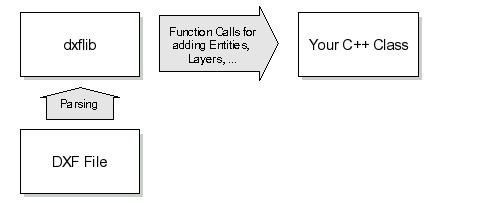
\includegraphics[scale=0.3]{images/dxf.png}
\caption{DXF working}
\end{figure}

\subsection{Group Codes}
The group code is an integer which implicitly defines the value type and acts as a key for the value. In ASCII DXF, group codes and values are written in a single line each.\\
Each group code listed in the DXF reference topics is presented by a numeric
group code value and a description. All group codes can apply to DXF files,
applications (AutoLISP or ObjectARX), or both. When the description of a code
is different for applications and DXF files (or applies to only one or the other),
the description is preceded by the following indicators:\\
\begin{itemize}
\item APP. Application-specific description.
\item DXF. DXF file-specific description.
\end{itemize}

\subsection{DXF CLASSES Section}
The CLASSES section in DXF files holds the information for application-defined
classes whose instances appear in the BLOCKS, ENTITIES, and OBJECTS sections
of the database. It is assumed that a class definition is permanently fixed in the
class hierarchy.

\subsection{DXF TABLES Section}
The group codes described in this chapter are found in DXF TM files and used by
applications. The TABLES section contains several tables, each of which can
contain a variable number of entries. These codes are also used by AutoLISP
and ObjectARX applications in entity definition lists.

\subsection{Introduction to \LaTeX}
\image{0.2}{images/latex.png}{\LaTeX{} Logo}
\LaTeX{}, I had never heard about this term before doing this project,
but when I came to know about it's features, it is just excellent. 
\LaTeX (pronounced /ˈleɪtɛk/, /ˈleɪtɛx/, /ˈlɑːtɛx/, or /ˈlɑːtɛk/) is a 
document markup language and document preparation system for the \TeX{} 
typesetting  program. Within the typesetting system, its name is styled 
as \LaTeX.
\image{0.4}{images/donald.jpg}{Donald Knuth, Inventor Of \TeX{} typesetting system}
\hspace{-1.8em} Within the typesetting system, its name is styled as \LaTeX. The term 
\LaTeX{} refers only to the language in which documents are written, 
not to the editor used to write those documents. In order to create a 
document in \LaTeX, a .tex file must be created using some form of text 
editor. While most text editors can be used to create a \LaTeX{} document, 
a number of editors have been created specifically for working with \LaTeX.

\LaTeX{} is most widely used by mathematicians, scientists, 
engineers, philosophers, linguists, economists and other scholars in 
academia. As a primary or intermediate format, e.g., translating DocBook 
and other XML-based formats to PDF, \LaTeX{} is used because of the 
high quality of typesetting achievable by \TeX. The typesetting system 
offers programmable desktop publishing features and extensive facilities 
for automating most aspects of typesetting and desktop publishing, 
including numbering and cross-referencing, tables and figures, 
page layout and bibliographies.

\LaTeX{} is intended to provide a high-level language that
accesses the power of \TeX. \LaTeX{} essentially comprises a
collection of \TeX{} macros and a program to process \LaTeX documents. 
Because the \TeX{} formatting commands are very low-level, it is usually 
much simpler for end-users to use \LaTeX{}.

\subsection{Installing \LaTeX{} on System}
Installation of \LaTeX{} on personal system is quite easy. As i have used \LaTeX{} on Ubuntu 13.04 so i am discussing the installation steps for Ubuntu 13.04 here:
\begin{itemize}
\item Go to terminal and type\\\\
\textit{sudo apt-get install texlive-full}
\item Your Latex will be installed on your system and you can check for manual page by typing.\\\\
\textit{man latex}\\
in terminal which gives manual for latex command.\\
\item To do very next step now one should stick this to mind that the document which one is going to produce is written in any type of editor whether it may be your most common usable editor Gedit or you can use vim by installing first vim into your system using command.\\\\
\textit{sudo apt-get install vim}\\
\item After you have written your document it is to be embedded with some set of commands that Latex uses so as to give a structure to your document. Note that whenever you wish your document to be looked into some other style just change these set of commands.\\\\
\item When you have done all these things save your piece of code with .tex format say test.tex. Go to terminal and type\\\\
\textit{latex path of the file test.tex Or pdflatex path of the file test.tex\\ eg: pdflatex test.tex}\\
for producing pdf file simultaneously.\\
After compiling it type command\\\\
\textit{evince filename.pdf\\ eg: evince test.pdf}\\
To see output pdf file. 
\end{itemize}

\subsection{Regular Expression}
A regular expression processor translates a regular expression into a nondeterministic finite automaton (NFA), which is then made deterministic and run on the target text string to recognize substrings that match the regular expression. Regular expressions are so useful in computing that the various systems to specify regular expressions have evolved to provide both a basic and extended standard for the grammar and syntax; modern regular expressions heavily augment the standard. Regular expression processors are found in several search engines, search and replace dialogs of several word processors and text editors, and in the command lines of text processing utilities, such as sed and AWK.\\\\
\begin{figure} [h!]
\centering
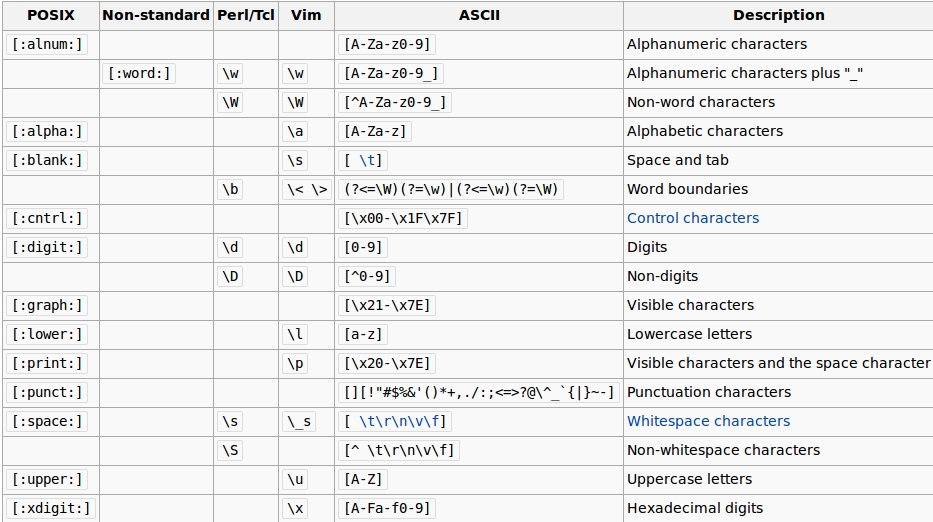
\includegraphics[scale=0.3]{images/regx.png}
\caption{meta classes}
\end{figure}

\subsection{Github}
The Git feature that really makes it stand apart from nearly every other Source Code
Management (SCM) out there is its branching model.Git allows and encourages you to
have multiple local branches that can be entirely independent of each other.The creation,
merging, and deletion of those lines of development takes seconds. This means that you
can do things like:\\\\

\begin{figure} [h]
\centering

\includegraphics[scale=0.3]{images/github.png}
\caption{Github logo}
\end{figure}

\begin{itemize}
\item Frictionless Context Switching. Create a branch to try out an idea, commit a few
times, switch back to where you branched from, apply a patch, switch back to where
you are experimenting, and merge it in.
\item Role-Based Codelines. Have a branch that always contains only what goes to pro-
duction, another that you merge work into for testing, and several smaller ones for
day to day work.
\item Feature Based Workflow. Create new branches for each new feature youre working
on so you can seamlessly switch back and forth between them, then delete each
branch when that feature gets merged into your main line.
\item Disposable Experimentation. Create a branch to experiment in, realize its not going
to work, and just delete it - abandoning the workwith nobody else ever seeing it
(even if youve pushed other branches in the meantime). Notably, when you push to
a remote repository, you do not have to push all of your branches. There are ways
to accomplish some of this with other systems, but the work involved is much more
difficult and error-prone. Git makes this process incredibly easy and it changes the
way most developers work when they learn it.
\end{itemize}

Firstly, You creates a repository on github. To add new files to the repository or add changed files to staged area:\\
\begin{itemize}
\item $ git init$
\item $ git status$
\item $ git add <files>$
\item $ git commit$
\item $ git commit -a$
\item $ git push origin$
\item $ git push origin master$
\item $ git fetch origin$
\end{itemize}

If you want to clone any repositry from github. FOllow these commands:
\begin{itemize}
\item cd nameofdirectory
\item git init
\item git clone forkedURL
\end{itemize}

\subsection{shell scripting}
\begin{itemize}
\item What is Bash?
\end{itemize}
Bash is a ‘Unix shell’: a command-line interface for interacting with the operating system. It is
widely available, being the default shell on many GNU/Linux distributions and on Mac OS X; and
ports exist for many other systems. It was created in the late 1980s by a programmer named Brian
Fox, working for the Free Software Foundation. It was intended as a free-software alternative to
the Bourne shell (in fact, its name is an acronym for ‘Bourne-again shell’), and it incorporates
all features of that shell, as well as new features such as integer arithmetic and in-process regular
expressions.
\begin{itemize}
\item What is Shell?
\end{itemize}
The shell is the program which actually processes commands and returns output. Most shells also
manage foreground and background processes, command history and command line editing. These
features (and many more) are standard in bash, the most common shell in modern linux systems.
\begin{itemize}
\item What is shell scripting?
\end{itemize}
In addition to the interactive mode, where the user types one command at a time, with immediate
execution and feedback, Bash (like many other shells) also has the ability to run an entire script of
commands, known as a Bash shell script” (or Bash script” or shell script” or just script”). A script
might contain just a very simple list of commands or even just a single command or it might contain
functions, loops, conditional constructs, and all the other hallmarks of imperative programming. In
ect, a Bash shell script is a computer program written in the Bash program- ming language. Shell scripting is the art of creating and maintaining such scripts. Shell scripts can be called from the
interactive command-line described above; or, they can be called from other parts of the system.\\
One script might be set to run when the system boots up; another might be set to run every weekday
at 2:30 AM; another might run whenever a user logs into the system. Shell scripts are commonly
used for many system administration tasks, such as performing disk backups, evaluating system
logs, and so on. They are also commonly used as installation scripts for complex programs.\\ They
are particularly suited to all of these because they allow complexity without requiring it: if a script
just needs to run two external programs, then it can be a two-line script, and if it needs all the power
and decision-making ability of a Turing-complete imperative programming language, then it can
have that as well.\\
\subsection{Lua- Programming Language}
Lua is a powerful, fast, lightweight, embeddable scripting language. Lua combines simple procedural syntax with powerful data description constructs based on associative arrays and extensible semantics. Lua is dynamically typed, runs by interpreting bytecode for a register-based virtual machine, and has automatic memory management with incremental garbage collection, making it ideal for configuration, scripting, and rapid prototyping.\\\\
Lua is free software distributed in source code. It may be used for any purpose, including commercial purposes, at absolutely no cost.All versions are available for download.  The current version is Lua 5.2 and its current release isLua 5.2.3. Lua has many features:
\begin{itemize}
\item LUA  is a proven, Robust language.
\item LUA  is fast.
\item LUA  is portable.
\item LUA  is embeddable.
\item LUA  is powerful, but simple.
\item LUA  is small.
\item LUA  is free.
\end{itemize}

\subsection{GIMP}

\begin{figure} [h]
\centering

\includegraphics[scale=0.08]{images/GIMP.jpg}
\caption{GIMP logo}
\end{figure}
GIMP is an acronym for GNU Image Manipulation Program. It is a freely distributed program for such tasks as photo retouching, image composition and image authoring.It has many capabilities. It can be used as a simple paint program, an expert quality photo retouching program, an online batch processing system, a mass production image renderer, an image format converter, etc. GIMP is expandable and extensible. It is designed to be augmented with plug-ins and extensions.\\

\subsection{Features:}
GIMP has tools used for image retouching and editing, free-form drawing, resizing, cropping, photo-montages, converting between different image formats, and more specialized tasks. Animated images such as GIF and MPEG files can be created using an animation plugin.\\
The developers and maintainers of GIMP strive to create a high-end free software graphics application for the editing and creation of original images, photos, icons, graphical elements of web pages, and art for user interface elements.\\\\
\begin{figure} [h]
\centering
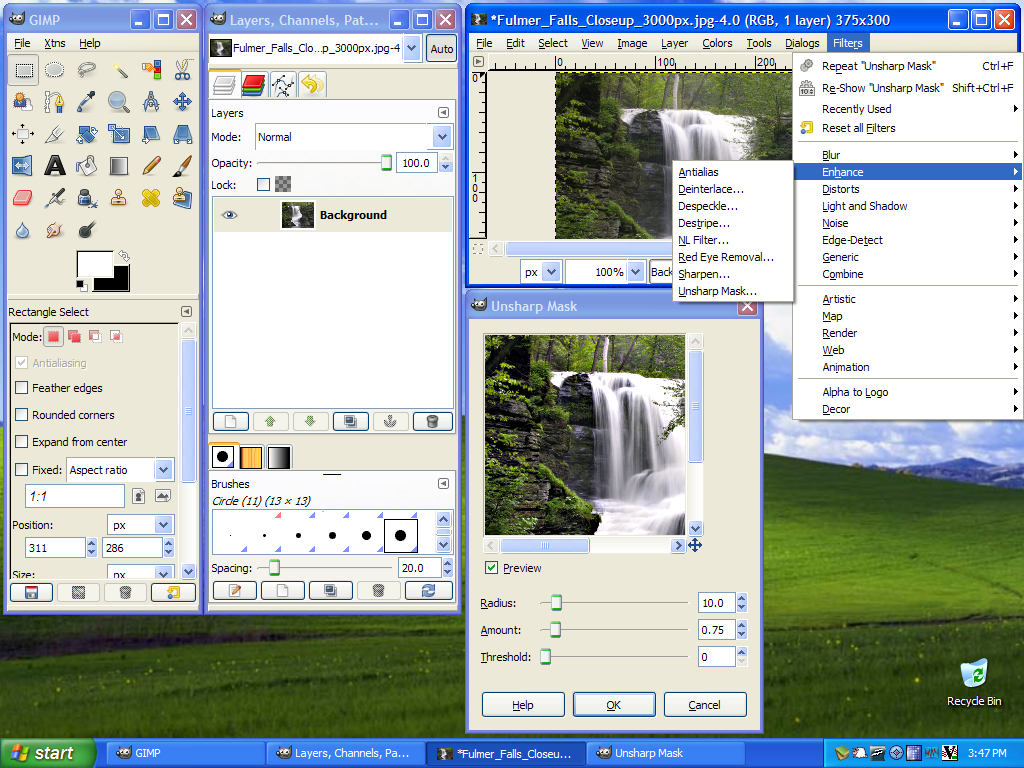
\includegraphics[scale=0.2]{images/feats.png}
\caption{GIMP FEATURES}
\end{figure}

\textbf{colour}
There are several ways of selecting colors including palettes, color choosers and using an eyedropper tool to select a color on the canvas. The built-in color choosers include RGB/HSV selector or scales, water-color selector, CMYK selector and a color-wheel selector. Colors can also be selected using hexadecimal color codes as used in HTML color selection. \\\\
\textbf{Selections and paths}
There are tools for creation of selections include a rectangular and circular selection tool, free select tool, and fuzzy select tool (also known as magic wand). More advanced selection tools include the select by color tool for selecting contiguous regions of color and the scissors select tool which creates selections semi-automatically between areas of highly contrasting colors.\\\\
\textbf{Image editing}
There are many tools that can be used for editing images in GIMP. The more common tools include a paint brush, pencil, airbrush, eraser and ink tools used to create new or blended pixels. Tools such as the bucket fill and blend tools are used to change large regions of space in an image and can be used to help blend images.A list of GIMP transform tools include the align tool, move, crop, rotate, scale, shear, perspective and flip tools.\\\\
\textbf{Layers, layer masks and channels}
An image being edited in GIMP can consist of many layers in a stack. The user manual suggests that "A good way to visualize a GIMP image is as a stack of transparencies," where in GIMP terminology, each transparency is a layer. This channel measures opacity where a whole or part of an image can be completely visible, partially visible or invisible.\\\\
\textbf{File formats}
\begin{enumerate}
\item Import and export: GIMP has import and export support for image formats such as BMP, JPEG, PNG, GIF and TIFF, along with the file formats of several other applications such as Autodesk flic animations, Corel Paint Shop Pro images, and Adobe Photoshop documents. Other formats with read/write support include PostScript documents, X bitmap image and Zsoft PCX. \item Import only: GIMP can import Adobe PDF documents and the raw image formats used by many digital cameras, but cannot save to these formats. An open source plug-in, UFRaw, adds full raw compatibility, and has been noted for being quicker than Adobe in updating for new camera models, several times.
\end{enumerate}

\section{Coding standards of Language used} % (fold)
\label{sec:coding_standards_of_language_used}

\begin{enumerate}
\item \textbf{Meaningful names of variables, classes and functions:} \\
The name of any variable, class or function should clearly imply what it does. Assigning a random name to any of these should not be done.\\
e.g. \textbf{myFunctionName()} is not a meaningful name.
\item \textbf{Spacing:}\\
Proper indentation and spacing is to be followed. 
\begin{enumerate}
\item No space should precede the comma.\\
e.g
\begin{verbatim}
func(a, b, c) // correct 
func(a ,b , c) // incorrect 
func(a , b,c) // incorrect
\end{verbatim}
\item While creating conditional blocks, say using \textbf{if} or \textbf{for} etc., a space should be there between the keyword and the opening parenthesis that follows.\\
e.g
\begin{verbatim}
if (condition)  // correct  
if(condition)// incorrect
\end{verbatim}
\item Creating a class should look like\\\\
\begin{verbatim}
className : public inheritedClass{
   //class definition
 };
\end{verbatim}
Keeping a space before and after the colon is advised and curly brace must start after the class name.
\end{enumerate}
\item \textbf{camel-Casing:}\\
The naming standard for names to be followed is camel-Casing.\\
e.g
\begin{verbatim}
functionName     
className  
variableName 
\end{verbatim}
\item \textbf{Defining if-else blocks:}\\
A line between \textbf{if} and \textbf{else} blocks: An empty line must be there between if and else blocks if each contains multiple statements. Otherwise, this empty line can be avoided.\\
e.g
\begin{verbatim}
if (condition) {    
  /**
  * do something  
  * do more 
  */  
} else {  
  /**
  * do something  
  * do more 
  */  
}
\end{verbatim}
Or it can be like: 
\begin{verbatim}
if (condition)    
  // do something  
else  
  // do something 
\end{verbatim}
\end{enumerate}

% section coding_standards_of_language_used (end)

\section{Project Scheduling} % (fold)
\label{sec:project_scheduling_}
Scheduling the project tasks is an important project planning activity. Software project scheduling is an activity that distributes estimated effort across the planed project duration by allocating the effort to specific software engineering tasks.\\\\
In project management, a schedule is a listing of a project's milestones, activities, and deliverables, usually with intended start and finish dates. Those items are often estimated in terms of resource allocation, budget and duration, linked by dependencies and scheduled events. A schedule is commonly used in project planning and project portfolio management parts of project management. Elements on a schedule may be closely related to the work breakdown structure.\\\\
Before a project schedule can be created, the schedule maker should have a work breakdown structure (WBS), an effort estimate for each task, and a resource list with availability for each resource.\\\\
In order to schedule the project, activities, a software project needs to the following:
\begin{enumerate}
\item Identify all the tasks needed to complete the project
\item Break down large tasks into small activities
\item Determine the dependency among different activities
\item Establish the time duration for completing the various activities
\item Plan starting and ending date for completing the various activities
\end{enumerate}
Various tools that are used for Project scheduling are Gannt Charts or PERT Chats.
\subsection{Gantt Charts}
A Gantt chart, commonly used in project management, is one of the most popular and useful ways of showing activities (tasks or events) displayed against time. On the left of the chart is a list of the activities and along the top is a suitable time scale. Each activity is represented by a bar; the position and length of the bar reflects the start date, duration and end date of the activity. This allows you to see at a glance:
\begin{enumerate}
\item What the various activities are
\item When each activity begins and ends
\item How long each activity is scheduled to last
\item Where activities overlap with other activities, and by how much
\item The start and end date of the whole project
\end{enumerate}
\vspace*{1cm}
\begin{figure}[!h]
\begin{center}
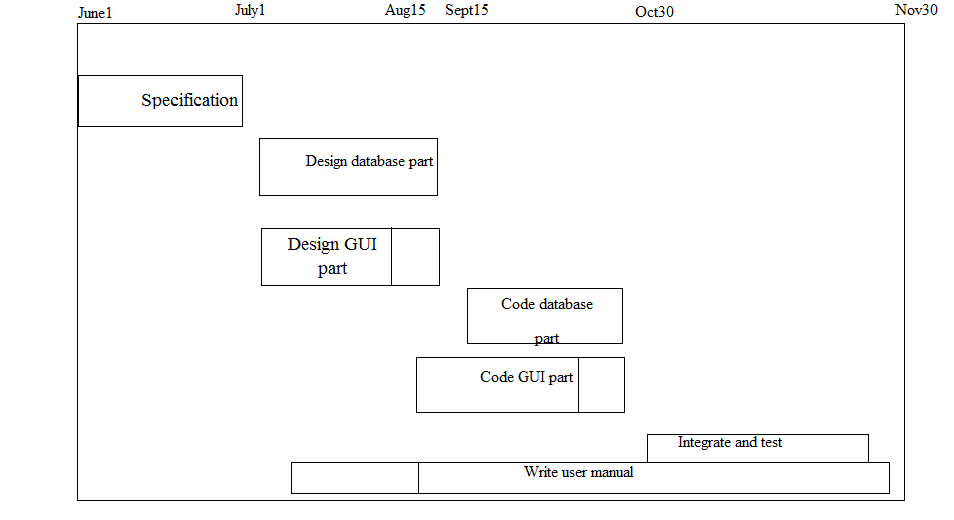
\includegraphics[scale=0.4]{images/ganttchart.png}
\end{center}
\caption{Gannt Chart}
\end{figure}
\subsection{PERT Chart}
The program (or project) evaluation and review technique, commonly abbreviated PERT, is a statistical tool, used in project management, which was designed to analyze and represent the tasks involved in completing a given project.PERT is a method to analyze the involved tasks in completing a given project, especially the time needed to complete each task, and to identify the minimum time needed to complete the total project.\\\\
PERT was developed primarily to simplify the planning and scheduling of large and complex projects. It was developed for the U.S. Navy Special Projects Office in 1957 to support the U.S. Navy's Polaris nuclear submarine project. It was able to incorporate uncertainty by making it possible to schedule a project while not knowing precisely the details and durations of all the activities. It is more of an event-oriented technique rather than start- and completion-oriented, and is used more in projects where time is the major factor rather than cost. It is applied to very large-scale, one-time, complex, non-routine infrastructure and Research and Development projects.
\begin{figure}[!h]
\begin{center}
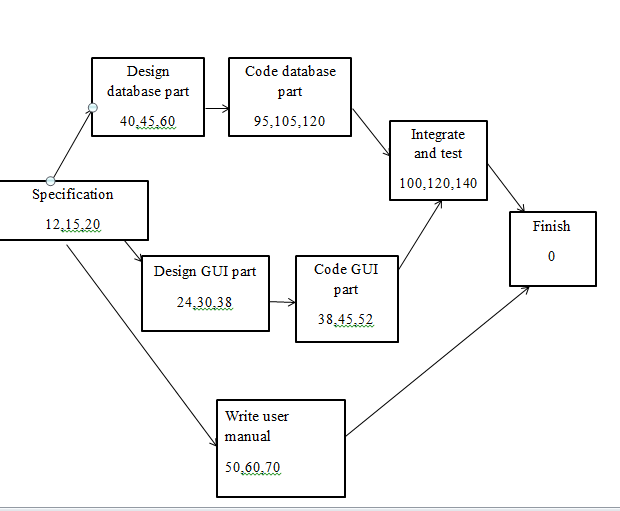
\includegraphics[scale=0.4]{images/pert.png}
\end{center}
\caption{Pert Chart}
\end{figure}
% section project_scheduling_ (end)

\section{Testing Techniques and Test Plans} % (fold)
\label{sec:testing_techniques_and_test_plans}
System testing validates software once it has been incorporated into a larger system Software is incorporated with other system elements and a series of system integration and validation tests are conducted .System testing is actually a series of different tests whose primary purpose is to fully exercise the computer based system.Once the system has been developed it has to be tested. In the present system we have to take care of valid property and assessment numbers i.e. there should not exists any duplicate number in each case. Care should betaken that the appropriate data is retrieved in response to the queries. The main thing, which should be considered, is the user interface. We have to see whether the user finds any difficulty in executing the system.Necessary messages and prompts should appear as needed to necessitate the users and make him alert if the invalid actions and help him to redo the required action. All the above cases any more are tested by providing the required data as input to the system so that any more tested by providing the required data as input to the system so that any uncovered errors can be traced out. For unit testing, we rested each module, as they are working well independently, went for integration testing. We integrated all the modules and after integration also they gave same results. For validation we checked for all different type of inputs and they gave correct results, and did the total process will satisfy the total validations that will checked and find out the results.
\begin{enumerate}
\item \textbf{The Data type Input Testing} 
\begin{itemize}
  \item \textbf{String Test Case} : It is the test case in which there is an insertion of string records in a text box.
    \begin{enumerate}
      \item A-Z alphabet acceptance testing: in a string test case, we can enter only alphabets (a-z) in a textbox. 
      \item Number testing: cannot enter numerals in string test case. 
      \item Blank Space testing: cannot enter blank spaces. 
      \item Maximum length: cannot enter more than 50 characters.
    \end{enumerate}
  \item \textbf{Numeral Test Case} : There is an insertion of numbers ranging from 0-9 in the text box.
    \begin{enumerate}
      \item 0-9 number acceptance testing: The numbers 0-9 can only enter in the text box. 
      \item A-Z alphabet testing: cannot enter alphabets (a-z) in number test case. 
      \item Blank Space testing: cannot put blank spaces in number text box. 
      \item Length of integer testing: The numerals in a text box are restricted by a specific maximum length for a specific field. Maximum length for Phone (cell, home) = 10
    \end{enumerate}
  \item \textbf{Boolean Test case} : It is a testing of check boxes which are to be set either true or false.
  \item \textbf{String, Number and Symbol Test case} : It is a test case consists of entry of all the data types like string, number and symbols, etc.
  \item \textbf{Date input Test Case} : when the text box is to be entered with date, then this testing is used.
    \begin{enumerate}
      \item 5.1. Due (Before) date testing: When the date entered is to be the date less than the today’s date. 
      \item After Date testing: When the date entered is to be the date after the today’s date. 
      \item  Current date Testing: When the date entered is to be the current date only. 
    \end{enumerate}     
\end{itemize}
\item \textbf{CRUD Operations Testing} : Its testing of create, read, update, delete operations.
    \begin{enumerate}
\item \textbf{Save} : It is to test the successful saving operation of record in any part of the software.
\item \textbf{Update} : It is to test the update/editing operation of records in any part of software. 
\item \textbf{Delete} : This test is to check the delete operation in the software. 
\item \textbf{Retrieval} : This test case is to check the successful retrieval of data and records on clicking of any link.
    \end{enumerate}
\end{enumerate}
% section testing_techniques_and_test_plans (end)
